\documentclass{article}   	% use "amsart" instead of "article" for AMSLaTeX format
\usepackage{geometry}                		% See geometry.pdf to learn the layout options. There are lots.
\geometry{letterpaper}                   		% ... or a4paper or a5paper or ... 
%\geometry{landscape}                		% Activate for rotated page geometry

\usepackage[parfill]{parskip} 				% Activate to begin paragraphs with an empty line rather 
\usepackage{graphicx}				% Use pdf, png, jpg, or eps§ with pdflatex; use eps in DVI 
\usepackage{amssymb}
\usepackage{amsmath}
\usepackage{mathtools}
\usepackage{bbm}


\newcommand{\summ}{\frac{1}{N}\sum_{i=1}^{N}}
\newcommand{\bw}{\mathbf{w}}
\newcommand{\bx}{\mathbf{x}}
\newcommand{\lra}{\Leftrightarrow}
\newcommand{\1}{\mathbbm{1}}
\newcommand{\E}{\mathbbm{E}}
\newcommand{\Prob}{\mathbbm{P}} 
\newcommand{\itt}{\intertext}

\title{Assignment 2}
\author{Jeppe Johansen}

\begin{document}
\maketitle

%%%%%%%%%%%%%%%%%%%%%%%%%%
%%%%%%%%%%%%%%%%%%%%%%%%%%


	% Exercise 1


%%%%%%%%%%%%%%%%%%%%%%%%%%
%%%%%%%%%%%%%%%%%%%%%%%%%%

\section{Illustration of Hoeffding's Inequality}

\subsection*{1}


The implementation of the coin flips is made the following way. Using a binomial distribution (repeated bernoulli distribution), with $\mu=0.5, n=20$ times $1000000$ I get the right distribution. This can be considered a $20 \times 1000000$ matrix.

\subsection*{2}

Below is the plot of the frequencies. of getting $P(\summ X\geq \alpha), \alpha \in  \left[ 0.5, 0.55, \ldots , 0.95, 1 \right] $ and $N=20$. As the figure shows the probability decreases as the right hand side of a normal distribution. This is not a surprise however, since the central limit theorem ensures that the parameter space $\theta$ is normally distributed. Here it's noted that $\theta$ is the empirical average.



It's noted
\begin{figure}
    \centering 
    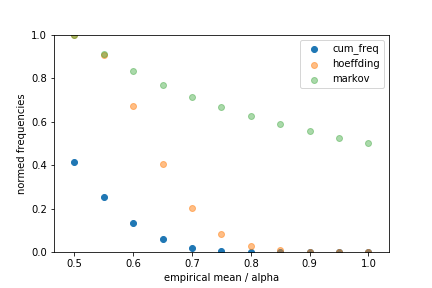
\includegraphics{figs/ex1.png}
    \caption{Distributions of $Z$}
    \label{fig:ex2}
\end{figure}

\subsection*{3}
It's not necessary to add any more granularity to the distribution of alpha, since the empirical average og 20 coin flips cannot take any discrete value inbetween the given alphas. This follows clearly from this example: Assume 20 coin flips with 10 heads and 10 tails. In this case the empirical average would be $0.5$. Now assume that in the next 20 coin flips there will be 11 heads and 9 tails. This would lead to the empirical average of $0.55$, which imply a granularity of $0.05$

\subsection*{6}
Looking at figure \ref{fig:ex2} Hoeffding's  bound and markov's bound is plotted next to the values of frequencies of observed empirical averages above 5. First it's noted that the sharpest decline happens in the frequencies of the empirical averages. This is totally expected, since both Markov's and Hoeffding's bound should be an upper limit of a given observed frequency of the empirical average. Next it's noted that hoeffdings bound declines much faster that the Markov bound. This has the implication, that Hoeffding's bound is a better way to bound probability that Markov's bound, since, when bounding probability it's prefered that have as hard a bound as possible, to get a sense of the possible outcomes of a given random process. Lastly it can be seen that Markov's bound decrease way slower than Hoeffding's bound, however it still does bound the probability space.

\subsection*{7}

The exact probability is calculated the following way $N=20$:

\begin{align*}
	\Prob \left\{�\summ X_{i} \geq = 1 \right\} &= \prod_{i=1}^{N}\frac{1}{2} = 9.537 \times 10^{-7} \\
\intertext{The probability that the empirical average is larger or equal to $0.95$}
	\Prob \left\{�\summ X_{i} \geq =0.95 \right\} &= \sum_{\alpha \in \{0.95, 1\} } \Prob(X \geq \alpha) =  2.003 \times 10^{-5}
\intertext{The hoefding's bounds  $HB$ is calculated below:}
	HB(\alpha=1.00, \mu=0.5, N=20) &= 4.540 \times 10^{-5} \\
	HB(\alpha=0.95, \mu=0.5, N=20) &= 0.0003035
\intertext{The Markov's bounds $MB$ is calculated below:}
	MB(\alpha=1.00, \mu=0.5, N=20) &= 0.5 \\
	MB(\alpha=1.00, \mu=0.5, N=20) &= 0.526
\end{align*}

%%%%%%%%%%%%%%%%%

		% Exercise 2

%%%%%%%%%%%%%%%%%


\section{The effect of scale (range) and normalization of random variables in Hoeffding?s inequality}

From the Theorem of Hoeffding's Inequality I get:
\begin{align}
	&\Prob \left\{ �\sum_{i}^{N}X_{i} - \sum_{i}^{N} \E \left[ � X_{i} \right] \geq \epsilon \right\} \leq e^{-2\epsilon / �\sum_{i}^{N}(b_{i} - a_{i})^{2}} 
	\intertext{Since I know we are looking at discrete data (people either arriving or not I know: $\Prob \{X_{i} \in [0,1] \} = 1$ and $\E[X_{i}] = \mu$ for all observations. This implies:}
	&a_{i}=0 \land b_{i}= 1 \\
	\intertext{Using this I rewrite:}
	&\Prob \left\{ �\sum_{i}^{N} X_{i} -  \sum_{i}^{N} \E \left[ � X_{i} \right] \geq \epsilon \right\} \leq e^{-2\epsilon / 		N } 
	\intertext{DIviding through by $n$ yields:}
	&\Prob \left\{ \summ X_{i} -  \summ \E \left[  X_{i} \right] \geq  \frac{1}{N} \epsilon \right\} \leq e^{-2\epsilon / 		N } \\ 
	= \quad &\Prob \left\{ \summ X_{i} - \E \left[  X_{i} \right] \geq  \frac{1}{N} \epsilon \right\} \leq e^{-2\epsilon / 		N }
	\intertext {Now it's clear that epsilon ca be redefined: $\hat{\epsilon} = \epsilon \frac{1}{N}$ } 
	 &\Prob \left\{ \summ X_{i} - \E \left[  X_{i} \right] \geq  \hat{\epsilon} \right\} \leq e^{-2 n \hat{\epsilon}} 
	\intertext{ Which was the result wanted ( corollary 2.4 )}
\end{align}



%%%%%%%%%%%%%%%%%

		% Exercise 3

%%%%%%%%%%%%%%%%%

\section{Probability in Practice}

\subsection{1}
An airline has 99 seats in the plane. We know they sell 100 tickets. The probability of not showing up i equal 0.05 which implies $\Prob [Showing up]= 0.95$ since there is only 1 way that over 99 people can board the plane we can calculate the bounds. 
\begin{align}
	\Prob�\left\{ X>99 \right\} = \Prob \left\{ X\geq100 \right\} = \prod_{i=1}^{100} 0.95 &= 0.00592 \qquad 
\intertext{Furthermore the Hoeefding's bound is found:}
	\Prob \left\{ \summ \geq \underset{\epsilon}{\underbrace{\alpha - \mu}} = 1 - 0.95 \right\} \leq e^{2n\epsilon^{2}}  &= 0.6065 \qquad N=100
\intertext{Lastly the Markov's bound is found}
	\Prob \left\{ \summ \geq \epsilon = 1 \right\} \leq \frac{\E[X] }{\epsilon} &= \frac{0.95}{1} \qquad N=100
\end{align}

\subsection{2}

We have to different set of information given. That empirically we found that 9500 out of 10000 guests arrive, and we know that we have overbooked if all passengers arrive to a given plane. We have from 3.1 already found that the probability of a plane being overbooked can be described as $p^{100}$ where 100 denote the number of passengers. I optimize the function by knowing that these to probabilities are independent that is the probability of observing 9500 out of 10000 people getting to their plane and all 100 arriving to one giving plane. Using this information we use the hoeffding bound for the probability of 9500 arriving to a plane. When this bound is found i multiply it with the probability that i a plane gets overbooked. Then i solve for $p$ and find the bound.

\begin{align}
	&\Prob \left( \sum_{i=1}^{10000} X_{i} \geq 9500 \right) \\
	= &\Prob \left( \sum_{i=1}^{10000} X_{i} - 10000\cdot p \geq 9500 - 10000\cdot p \right)  \\
	\leq &e^{-2(10000(0.95-p))^2 / \sum_{i=1}^{10000}(b_{i} - a_{i})^{2}} \\
	=& \leq e^{-2(10000(0.95-p))^2 / \sum_{i=1}^{10000}(0 - 1)^{2}} \\
	=&  \leq e^{-2(10000(0.95-p))^2 / \sum_{i=1}^{10000}1} \\
	=&  \leq e^{-2(10000(0.95-p))^2 / 10000}
\intertext{Now using the expression for the probability (bound) of all people arriving to the plane $p^{100}$ the probability can be bound:}
	&p^{100}\cdot e^{-2(10000(0.95-p))^2 / \sum_{i=1}^{10000}1}  = 0.00619
\end{align}

Where the above equation is solved numerically. We find $p=0.954$ when the equation is solved numerically. The figure below (figure \ref{fig:ex2} shows the corresponding bound given probability $p$.

\begin{figure}
    \centering 
    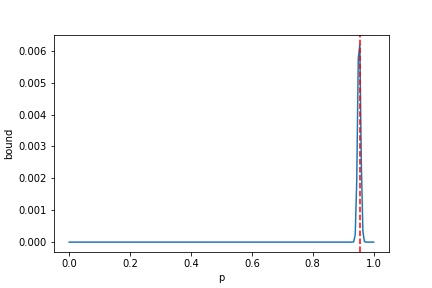
\includegraphics{figs/ex3.png}
    \caption{p and bound}
    \label{fig:ex2}
\end{figure}


%%%%%%%%%%%%%%%%%%%%%%

	% Logistic Regression

%%%%%%%%%%%%%%%%%%%%%%

\section{Logistic Regression}
\subsection{Cross entropy error measure}

\begin{align}
	min.  \qquad &\summ ln \left( \frac{1}{\theta(y_n \bw^{t} \bx_{n} )} \right) &= \qquad  \\
	\intertext{Using that $1 - \theta(s) = \theta(-s)$ I write:} 
	\theta(y,\bx , \bw) &= \1_{(y=1)}\theta(\bw^{t}\bx_{n}) +  \1_{(y=-1)}\theta(-\bw^{t} \bx_{n}) \\
	\theta(y,\bx , \bw) &= \1_{(y=1)}\theta(\bw^{t}\bx_{n}) +  \1_{(y=-1)}(1 - \theta(\bw^{t} \bx_{n})) \\
	\intertext{Substituting $\theta(y, \bw, \bx)$ with $h(x)$:}
	 &= \1_{(y=1)}\frac{1}{h(x)}+ \1_{(y=-1)}\frac{1}{1-h(x)}
	 \intertext{ now plugging this result in:�}
	min. \qquad  & \summ \left( \1_{(y=1)} ln \frac{1}{h(x)} + \1_{(y=-1)} ln \frac{1}{1 - h(x)}  \right) \\
	E_{(\bw)} &= \summ \left( \1_{(y=1)} ln \frac{1}{h(x)} + \1_{(y=-1)} ln \frac{1}{1 - h(x)}  \right)
\end{align}

\subsection{Logistic regression loss gradient}

\begin{align}
	\itt{Using the expression for $E_{in}(\bw)$ at equation $3.9$:}
	E_{in}(\bw) &= \summ ln (1+ e^{ -y_{n} \bw^{t} \bx_{n} }) \qquad \lra�\\
	\frac{\partial}{\partial \bw } &= \summ \frac{1}{1+ e^{ -y_{n} \bw^{t} \bx_{n} }} e^{ -y_{n} \bw^{t}\bx_{n} }(-y_{n}\bx_{n}) \\
	\frac{\partial}{\partial \bw }&= \nabla E_{in}(\bw) = \summ \frac{(-y_{n}\bx_{n})}{1+ e^{ y_{n} \bw^{t} \bx_{n} }}
	 \itt{First noting that:}
	 \theta(-s) &= 1 - \theta(s) = 1 - \frac{e^{s}}{1+e^{s}}  = \frac{e^{s} + 1 - e^{s}}{1+e^{s}} = \frac{1}{1+e^{s}} \\
	 \itt{using this expression we get:}
	 \nabla E_{in}(\bw) &= \summ \frac{1}{1+ e^{ y_{n} \bw^{t} \bx_{n} }} (-y_{n}\bx_{n}) \\
	  &= \summ \theta(y, \bw, \bx) (-y_{n}\bx_{n}) \\
\end{align}

\subsection{Logistic regression implementation}

The implementation of the logistic regression is made in the following way. Looking at $p. 95$ the algorithm for the logistic regression is written up. First i calculate the scalar using matrix manipulation. From there i use a while loop that runs until the gradient is sufficiently small, which implies the parameters has converged sufficiently. When parameters has converged the the unique minimum of the parameter space has been found. The loop goes the following way:
\begin{enumerate}
	\item Initialize weights $\bar{}0$ to the zero-vector.
	\item calculate the gradient as described above.
	\item recalculate the weights.
	\item feed the new weights into the algorithm
\end{enumerate}


\subsection{Iris Flower Datset}

In the iris flower dataset I implement the algorithm and get the following weigths in the test dataset:
\begin{enumerate}
	\item Length: $8.48$
	\item Width: $-50.84$
	\item Intercept: $-29.04$
\end{enumerate}

And the test error is: $\summ error = 0.61$ where error is $error \in \left\{ 0, 1 \right\}$ This is a quite poor performance, and could imply an error in the code. However after two different implementations of both the gradient-algorithm and the loop-algorithm, i must concede and conclude the algorithm just performs poorly.


\end{document}  